\documentclass[border=3pt]{standalone}
% Preâmbulo compartilhado pelos diagramas TikZ da aula 4 de Navegação (Representação de Mapas)
\usepackage[T1]{fontenc}
\usepackage[utf8]{inputenc}
\usepackage{lmodern}
\usepackage{amsmath}
\usepackage{xcolor}
\usepackage{tikz}
\usetikzlibrary{arrows.meta,angles,quotes,decorations.pathmorphing,decorations.pathreplacing,calc,
                positioning,shapes.geometric,shapes.misc,backgrounds,fit,
                math}

% Paleta (mesma dos SVGs originais)
\definecolor{dblue}{HTML}{2A5B8C}
\definecolor{dorange}{HTML}{B3541E}
\definecolor{dgreen}{HTML}{4A7C59}
\definecolor{dred}{HTML}{9C4B4B}
\definecolor{dcream}{HTML}{F4F1EA}
\definecolor{dshade}{HTML}{DDD7C9}

% Função gaussiana (não normalizada por padrão de escala visual)
\pgfmathdeclarefunction{gauss}{3}{%
  \pgfmathparse{1/(#3*sqrt(2*pi))*exp(-((#1-#2)^2)/(2*#3^2))}%
}

% Estilos comuns (prefixo d... para não colidir com chaves internas do pgf)
\tikzset{
  >={Stealth[length=2mm]},
  dguide/.style={gray!55, dashed, line width=0.4pt},
  daxis/.style={gray!60, line width=0.7pt, ->},
  dbody/.style={fill=black!3, draw=black!80, line width=1pt},
  dacc/.style={draw=dblue, line width=1pt},
  dlbl/.style={black!55, font=\small},
  dsub/.style={black!45, font=\footnotesize},
  dstate/.style={circle, draw=black!80, fill=dcream, line width=1pt,
                 minimum size=17mm, font=\large, inner sep=1pt},
  dobs/.style={circle, draw=black!80, fill=dshade, line width=1pt,
               minimum size=14mm, font=\large, inner sep=1pt},
  dbox/.style={rounded corners=2pt, draw=black!80, fill=dcream, line width=1pt,
               align=center, inner sep=6pt},
  dop/.style={circle, draw=black!80, fill=white, line width=1pt,
              minimum size=6mm, inner sep=0pt, font=\small},
  dtrans/.style={->, dblue, line width=1pt},
  dmeas/.style={->, dorange, line width=1pt},
  dcurve/.style={line width=1pt, dblue},
  dcurveb/.style={line width=1.4pt, dorange},
}

\begin{document}
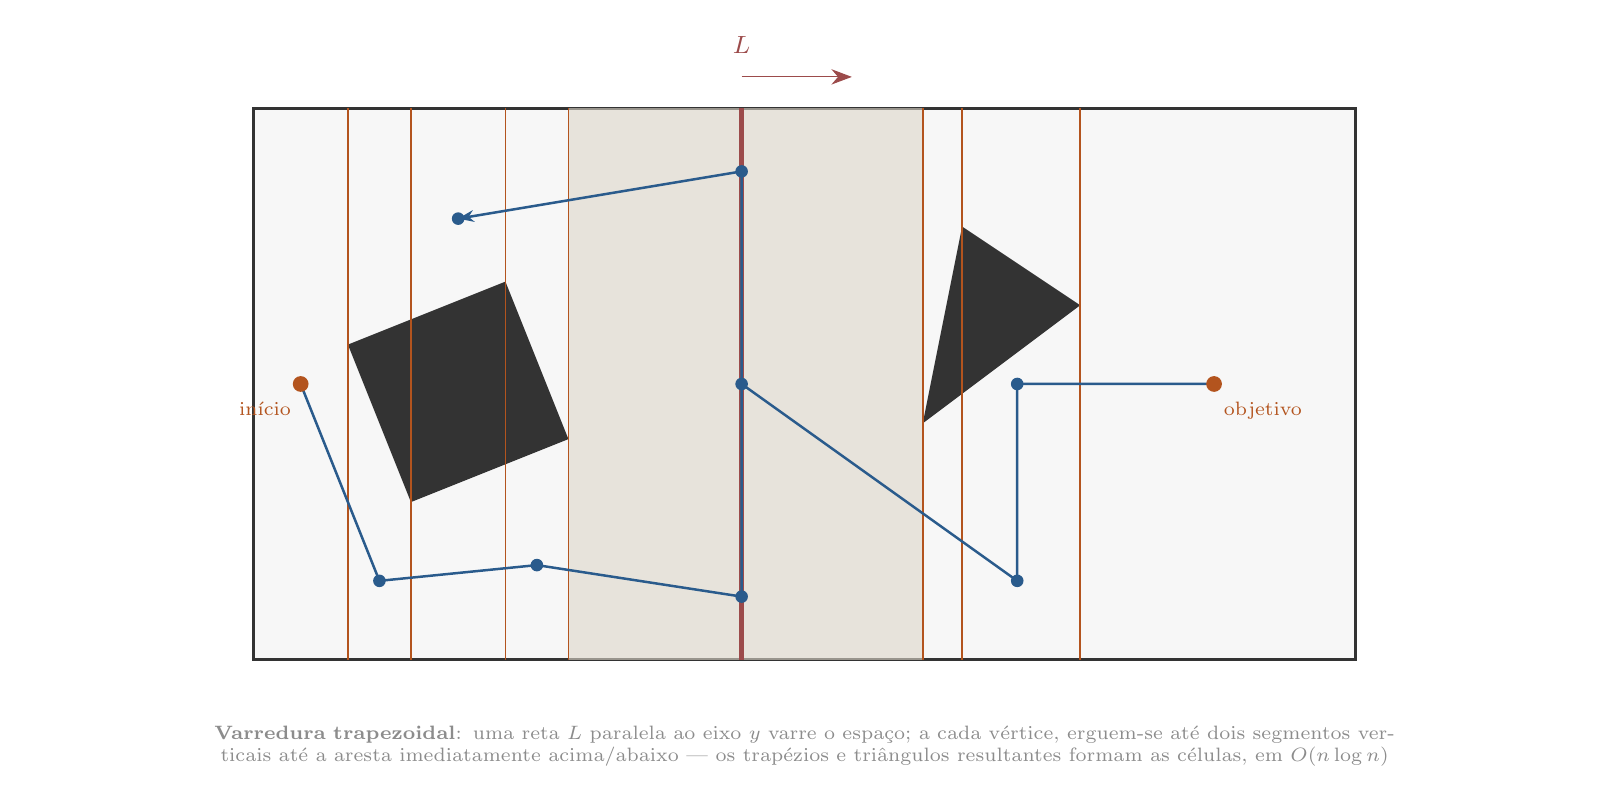
\begin{tikzpicture}[x=1cm,y=1cm]

  \draw[dbody, line width=1.2pt] (0,0) rectangle (14,7);

  % Faixa de exemplo (uma das colunas geradas pela varredura)
  \fill[dshade, opacity=0.6] (4.0,0) rectangle (8.5,7);

  % Obstáculos
  \fill[black!80] (2.0,2.0) -- (4.0,2.8) -- (3.2,4.8) -- (1.2,4.0) -- cycle;
  \fill[black!80] (8.5,3.0) -- (10.5,4.5) -- (9.0,5.5) -- cycle;

  % Segmentos verticais erguidos em cada vértice (varredura)
  \foreach \x in {1.2,2.0,3.2,4.0,8.5,9.0,10.5} {
    \draw[dorange, line width=0.6pt] (\x,0) -- (\x,7);
  }

  % Linha de varredura L em progresso, com seta de avanço
  \draw[dred, line width=1.6pt] (6.2,0) -- (6.2,7);
  \draw[dred, -{Stealth[length=2.6mm]}] (6.2,7.4) -- (7.6,7.4);
  \node[dred, font=\small] at (6.2,7.8) {$L$};

  % Grafo de conectividade sobre algumas células representativas
  \foreach \p in {(0.6,3.5),(1.6,1.0),(2.6,5.6),(3.6,1.2),(6.2,3.5),(6.2,6.2),(6.2,0.8),(9.7,3.5),(9.7,1.0),(12.2,3.5)} {
    \fill[dblue] \p circle (0.08);
  }
  \draw[dtrans, line width=0.9pt]
    (0.6,3.5) -- (1.6,1.0) -- (3.6,1.2) -- (6.2,0.8) -- (6.2,3.5) -- (9.7,1.0) -- (9.7,3.5) -- (12.2,3.5)
    (6.2,3.5) -- (6.2,6.2) -- (2.6,5.6);

  \fill[dorange] (0.6,3.5) circle (0.1);
  \node[dorange, font=\scriptsize, anchor=north east] at (0.6,3.4) {início};
  \fill[dorange] (12.2,3.5) circle (0.1);
  \node[dorange, font=\scriptsize, anchor=north west] at (12.2,3.4) {objetivo};

  \node[dsub, font=\scriptsize, align=center, text width=19.5cm] at (7,-1.1)
     {\textbf{Varredura trapezoidal}: uma reta $L$ paralela ao eixo $y$ varre o espaço; a cada vértice, erguem-se até dois segmentos verticais até a aresta imediatamente acima/abaixo --- os trapézios e triângulos resultantes formam as células, em $O(n \log n)$};

\end{tikzpicture}
\end{document}
